\chapter{Problemanalyse}
\textit{I dette kapitel analyses problemstillinger, som opstår i forbindelse med lægemiddelskift. Disse problemstillinger vil sammenfattes i en opsummering og afsluttes med en problemformulering, der danner fremadrettet grundlaget for rapporten.}

\section{Typer af lægemiddelskift}
Lægemiddelskift kan forekomme i forbindelse med kontraktskift eller ved restordre~\citep{Amgros2015}. Et årligt udbud foretages af Amgros, hvis der findes mere end én leverandør af lægemidlet. På denne måde bringes lægemidlerne i konkurrence, hvilket kan medføre et kontraktskift. I tilfælde af patent på lægemidlet er der ikke analog konkurrence, da prisen på lægemidlet ofte er fastsat. Restordre forekommer når efterspørgslen på et lægemiddel overstiger den tilgængelige mængde.~\citep{Amgros2015}. Udover kontraktskift og restordre kan bagatelkøb medføre præparatskift. Ved bagatelkøb er sygehusapoteket ikke forpligtet til at anvende lægemidlet og leverandøren omfattes ikke af indkøbs- eller forsyningspligt~\fxnote{\url{https://levportal.amgros.dk/Udbudsoversigt/Sider/Bagatelkob.aspx}}

\subsection{Kontraktskift}
Før et udbud finder sted har Amgros en dialog med medicinrådet~\citep{Amgros2017, Amgros2017a}. Lægemidlerne vurderes i forhold til effekt, eksisterende behandling og pris med det formål at stræbe efter laveste priser samt bedst mulig behandling for patienterne. Medicinrådet kategoriserer nye lægemidler og indikationer i forhold til den nuværende standardbehandling i stor, vigtig, lille eller ingen merværdi. Ud fra dette sammenstiller Amgros standardbehandlingen over for en omkostningsanalyse, der er udarbejdet af ansøgeren for lægemiddelskift. Amgros vurderer, hvorvidt de tilsendte oplysninger er relevante og valide. Den kliniske merværdi, omkostningsanalyse og estimeringen af budget konsekvenser danner grundlaget for prisforhandling. Medicinrådet beslutter efter prisforhandlingen, hvorvidt det nye lægemiddel skal anvendes som standardbehandling. Hvis dette er tilfældet foretages et kontraktskift.~\citep{Amgros2017, Amgros2017a}

\subsubsection{Udbudsprocessen}
*** KIG på 3.1 udbudsprocessen  ***

\subsection{Restordre}
Restordre kan forekomme på forskellige måder som f.eks. leveringesvigt, mangel på råvarer, forhindring i produktion, større forbrug af lægemidlet end beregnet eller at lægemidlet er solgt til en højere pris til et andet land~\citep{Amgros2017}. I tilfælde af restordre er det leverandørens ansvar at dække hospitalsapotekernes udgift ved indkøb af et erstatningslægemiddel~\fxnote{\url{https://levportal.amgros.dk/SiteCollectionDocuments/1.\%20Grundl\%C3\%A6ggende\%20information\%20om\%20l\%C3\%A6gemiddeludbud.pdf}}.


\section{Problematikker ved lægemiddelskift}
Der er både økonomiske og patientsikkerhedsmæssige konsekvenser ved et lægemiddelskift for så vidt angår restordre såvel som kontraktskift~\citep{Amgros2015}. Restordre er økonomisk omkostningsfuldt, da der skal foretages vareskift i systemer, på lagre og i medicinrum. Yderligere skal der gives behandlingsinstruktioner til hospitalsafdelingerne for at undgå fejl ved medicinering. Udover økonomiske faktorer udgør lægemiddelskift også patientsikkerhedsmæssige risici. Der kan opstå utilsigtede hændelser (UTH'er), hvis præparatet har skiftet navn, udseende og håndteringen af medicin er ændret.~\citep{Amgros2015}. 

De hyppigste årsager til UTH'er på de danske hospitaler skyldes i år 2013, 23,97~\%,medicinering, 20,86~\% kliniske processor, 17,98~\% kommunikation og dokumentation samt 17,23~\% administrative processer~\citep{Patientombuddet2013}. Antallet af rapporterede UTH'er i Region Nordjylland er steget med over 36\% fra år 2012 til 2014 ~\citep{Jensen2014}. Ud af 824 rapporterede UTH'er i år 2014 omhandlede 97\% medicinering, 86\% administration af medicin og 41\% at medicinen ikke var givet~\citep{Jensen2014}. 

\subsection{Kontraktskift}
De patientsikkerhedsmæssige konsekvenser opstået ved kontraktskift er undersøgt af et norsk studie~\citep{Hakonsen2010}. Interview med 100 sygeplejersker påviste at der opstod fejlmedicinering ved generiske lægemidler. Fejl i ordination og manglende dokumentation af lægemiddelskiftet af lægen blev opdaget af 46~\% sygeplejersker dagligt, hvorimod sygeplejerskerne altid fik lægemiddelsiftet dokumenteret. Yderligere følte 92~\% af sygeplejerskerne at generiske lægemidler var tidskrævende og 91~\% at disse øgede risikoen for fejl ved disponering.~\citep{Hakonsen2010}. De typiske hændelser ved kontraktskift fremgår af Figur \ref{fig:UTHkontraktskift}.

\begin{figure}[H]\centering
	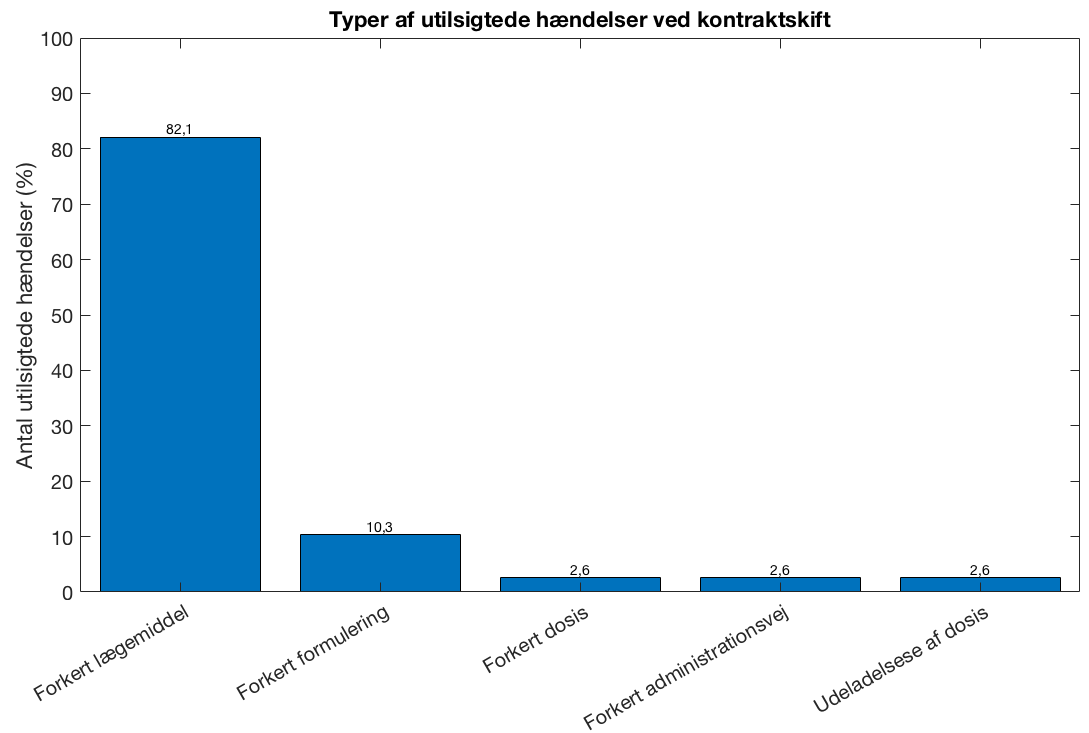
\includegraphics[width=0.7\textwidth]{billeder/UTH1.png} 
	\caption{Utilsigtede hændelser opstået ved kontraktskift\citep{Hakonsen2010}.}
	\label{fig:UTHkontraktskift}  
\end{figure}

Af Figur \ref{fig:UTHkontraktskift} fremgår det at 82,1~\% af UTH'erne forekommer ved disponering af forkert lægemiddel. Den næst hyppigste er forkert formulering \fxnote{hvad menes der med formulering?}


\subsection{Restordre}

*** KIG 3.5.5. Utilsigtede hændelser forårsaget af Restordre *** 16 PDF

De typiske hændelser ved restordre fremgår af Figur \ref{fig:UTHrestordre}.

\begin{figure}[H]\centering
	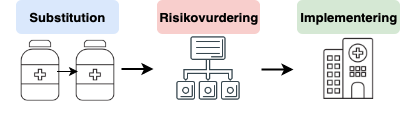
\includegraphics[width=1\textwidth]{billeder/forside.png} 
	\caption{Utilsigtede hændelser opstået ved restordre\citep{Hakonsen2010}.}
	\label{fig:UTHRestordre}  
\end{figure}


\section{Løsningsstartegier for problematikker}

\subsection{Kontraktskift}

\subsection{Restordre}
Disse risici kan mindskes ved instrukser og ændring af procedure på hospitalerne.
Tæt dialog med leverandøren.

*** SE 19Præparat ***

Jeg skal mere kigge på om det er muligt at gruppere de ting der skal gøres ved lægemiddelskift. Altså vejledninger. 


\section{Opsummering}
\subsection{Problemformulering}